\documentclass[preprint,12pt]{elsarticle}

%% Use the option review to obtain double line spacing
%% \documentclass[preprint,review,12pt]{elsarticle}

%% Use the options 1p,twocolumn; 3p; 3p,twocolumn; 5p; or 5p,twocolumn
%% for a journal layout:
%% \documentclass[final,1p,times]{elsarticle}
%% \documentclass[final,1p,times,twocolumn]{elsarticle}
%% \documentclass[final,3p,times]{elsarticle}
%% \documentclass[final,3p,times,twocolumn]{elsarticle}
%% \documentclass[final,5p,times]{elsarticle}
%% \documentclass[final,5p,times,twocolumn]{elsarticle}

%% The graphicx package provides the includegraphics command.
\usepackage{graphicx}
%% The amssymb package provides various useful mathematical symbols
\usepackage{amssymb}
%% The amsthm package provides extended theorem environments
%% \usepackage{amsthm}

%% The lineno packages adds line numbers. Start line numbering with
%% \begin{linenumbers}, end it with \end{linenumbers}. Or switch it on
%% for the whole article with \linenumbers after \end{frontmatter}.
\usepackage{lineno}
\usepackage{listings}
\usepackage[utf8]{inputenc}
%\usepackage[]{mcode}
%% natbib.sty is loaded by default. However, natbib options can be
%% provided with \biboptions{...} command. Following options are
%% valid:

%%   round  -  round parentheses are used (default)
%%   square -  square brackets are used   [option]
%%   curly  -  curly braces are used      {option}
%%   angle  -  angle brackets are used    <option>
%%   semicolon  -  multiple citations separated by semi-colon
%%   colon  - same as semicolon, an earlier confusion
%%   comma  -  separated by comma
%%   numbers-  selects numerical citations
%%   super  -  numerical citations as superscripts
%%   sort   -  sorts multiple citations according to order in ref. list
%%   sort&compress   -  like sort, but also compresses numerical citations
%%   compress - compresses without sorting
%%
%% \biboptions{comma,round}

% \biboptions{}

\journal{Journal Name}

\begin{document}

\begin{frontmatter}

%% Title, authors and addresses

\title{Decodificación de señales RBDS/RDS con GNURADIO}

%% use the tnoteref command within \title for footnotes;
%% use the tnotetext command for the associated footnote;
%% use the fnref command within \author or \address for footnotes;
%% use the fntext command for the associated footnote;
%% use the corref command within \author for corresponding author footnotes;
%% use the cortext command for the associated footnote;
%% use the ead command for the email address,
%% and the form \ead[url] for the home page:
%%
%% \title{Title\tnoteref{label1}}
%% \tnotetext[label1]{}
%% \author{Name\corref{cor1}\fnref{label2}}
%% \ead{email address}
%% \ead[url]{home page}
%% \fntext[label2]{}
%% \cortext[cor1]{}
%% \address{Address\fnref{label3}}
%% \fntext[label3]{}


%% use optional labels to link authors explicitly to addresses:
%% \author[label1,label2]{<author name>}
%% \address[label1]{<address>}
%% \address[label2]{<address>}

\author{Emmanuel Ortiz López}

%\address{California, United States}

\begin{abstract}
%% Text of abstract
Desarrollo de una aplicación Software Defined Radio basada en GNURADIO para sintonizar estaciones FM y desplegar la información RDS utilizando un receptor RTL-SDR
\end{abstract}

\begin{keyword}
SDR \sep GNURADIO \sep RDS
%% keywords here, in the form: keyword \sep keyword

%% MSC codes here, in the form: \MSC code \sep code
%% or \MSC[2008] code \sep code (2000 is the default)

\end{keyword}

\end{frontmatter}

%%
%% Start line numbering here if you want
%%
%\linenumbers

%% main text
\section{Software Defined Radio}
\label{S:1}
Radio Definido por Software (SDR por sus siglas en inglés) es una de las tendencias actuales en educación y diseño de sistemas de comunicaciones, la idea es usar un sistema mínimo de hardware (un receptor genérico) solo para capturar las señales de radio frecuencia (RF), y procesar la señal mediante software es decir modular, demodular, decodificar, etc. es decir sustituye la mayoría del hardware de los sistemas de comunicaciones.

\subsection{RTL-SDR}
Este es el nombre de los receptores de RF, existen varios modelos, en específico para este proyecto utilizamos RTL2832 este trabaja en las frecuencias de 24MHz hasta 1850MHz, funciona con todos los sistemas Operativos.\ref{rtl}

\begin{figure}[h]
\centering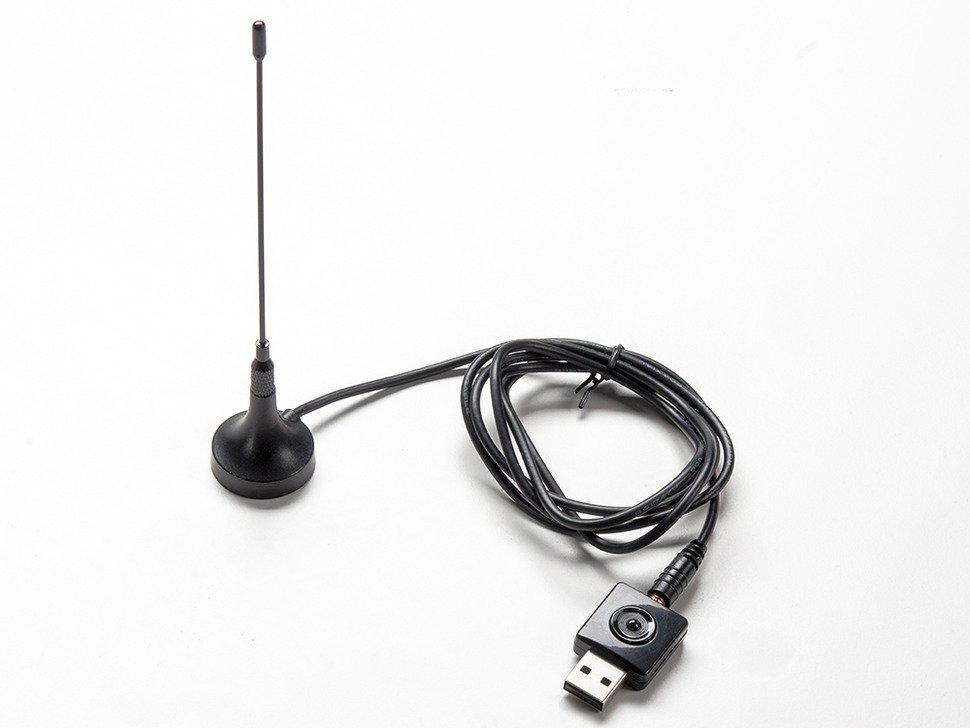
\includegraphics[width=0.2\linewidth]{RTL.jpg}
\caption{RTL2832}
\label{rtl}
\end{figure}


\subsection{GNURADIO}
 GNURADIO es un proyecto Open Source de GNURADIO Companion que ofrece un entorno grafico de programación a bloques. Estos bloque están basados en C++, Volk, qgrx, xml y Python Tiene 2 modalidades: front y back end a través del GUI de bloques, y creación back end. Existe la posibilidad de crear tus propios bloques para el entorno gráfico.
\begin{figure}[h]
\centering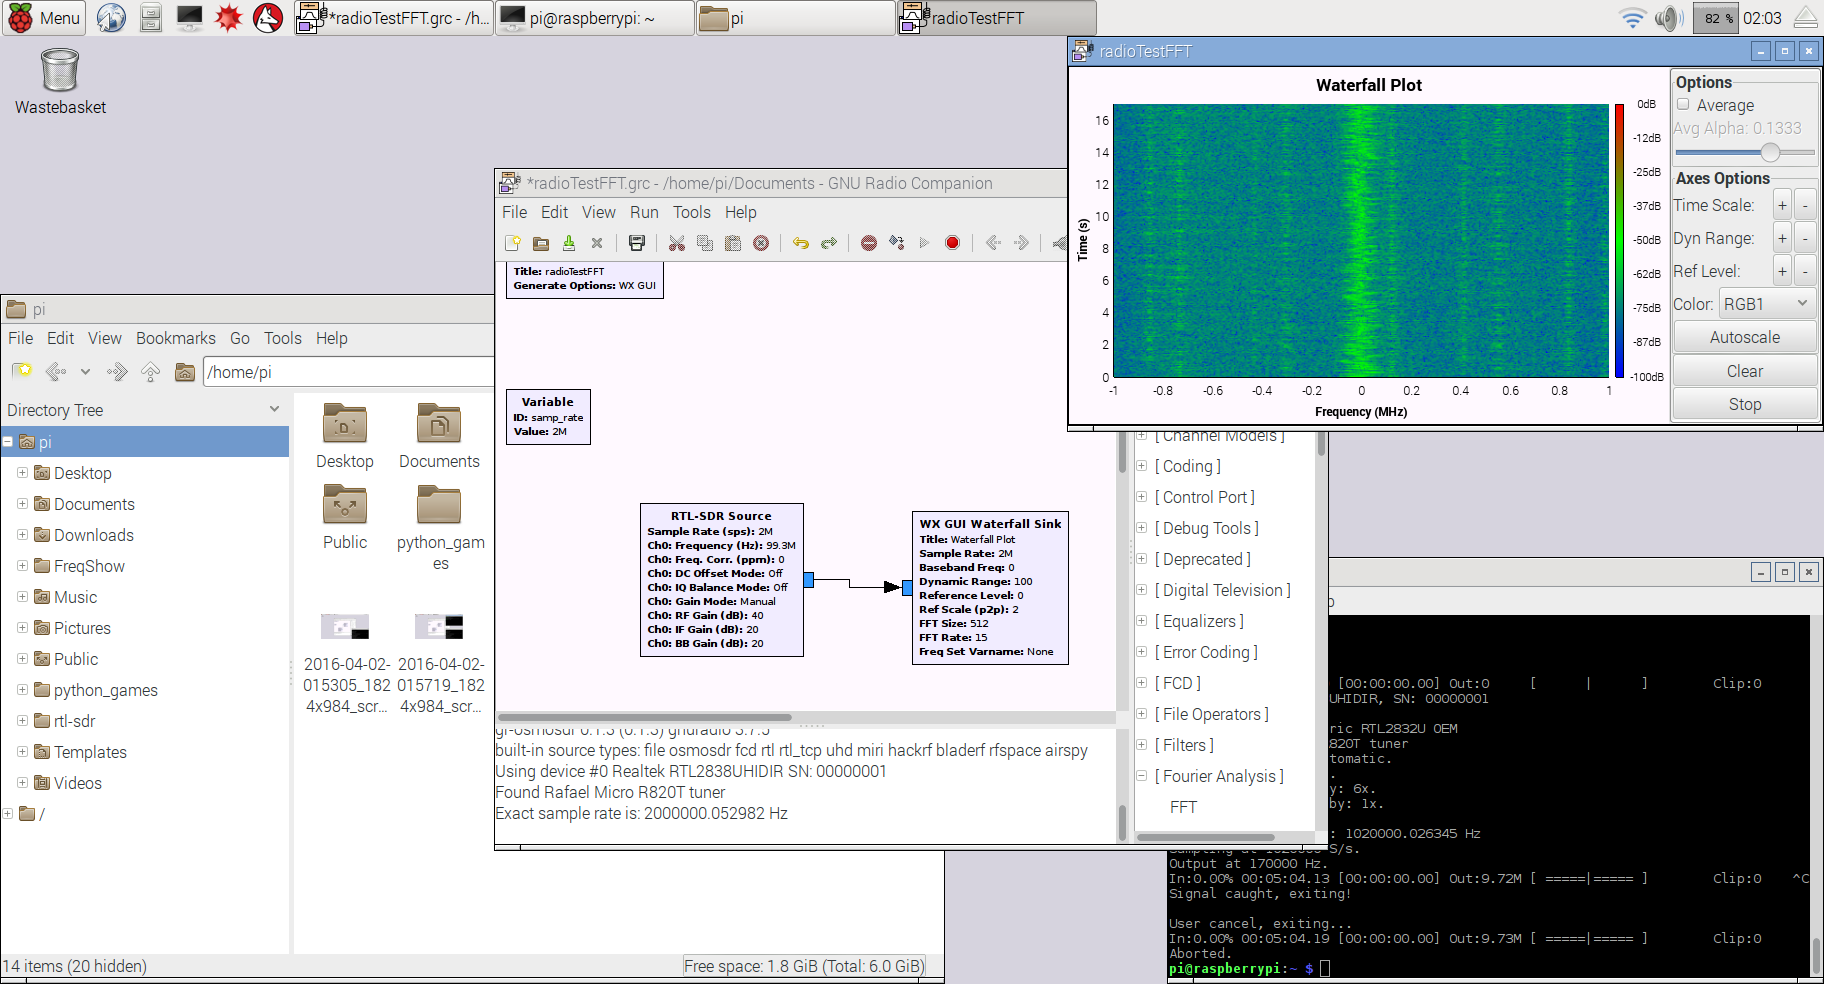
\includegraphics[width=0.4\linewidth]{2016-04-02-020310_1824x984_scrot.png}
\caption{Ejemplo de GNURADIO}
\label{rtl}
\end{figure}


%\begin{table}[h]
%\centering
%\begin{tabular}{l l l}
%\hline
%\textbf{Treatments} & \textbf{Response 1} & \textbf{Response 2}\\
%\hline
%Treatment 1 & 0.0003262 & 0.562 \\
%Treatment 2 & 0.0015681 & 0.910 \\
%Treatment 3 & 0.0009271 & 0.296 \\
%\hline
%\end{tabular}
%\caption{Table caption}
%\end{table}



%\begin{figure}[h]
%\centering\includegraphics[width=0.4\linewidth]{placeholder}
%\caption{Figure caption}
%\end{figure}
%

%
%\begin{equation}
%\label{eq:emc}
%e = mc^2
%\end{equation}

\section{Radio Data System}
\label{S:2}

Es un esquema de modulación para transmitir un estándar de datos utilizando las transmisiones FM, RDS por sus siglas en ingles fue creado por la Unión Europea de Radiodifusión. Estos datos son inaudibles pero contienen información como nombre de la estación, nombre de la canción hasta el informe de tráfico. Esta información vienen en una soportadora de 57 KHz que está en el ancho de banda de la transmisión FM, es una señal digital codificada en “Manchester”


\begin{figure}[htbp!]
\centering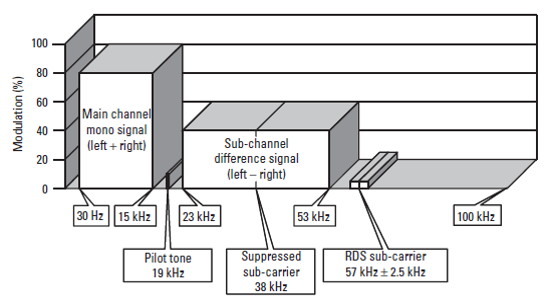
\includegraphics[width=0.4\linewidth]{fftRDS.png}
\caption{FFT de la señal FM-RDS}
\label{freqRDS}
\end{figure}
En específico la información que contiene son 104 bits, dividido en paquetes de 26 bits, 16 de estos son información el resto son bits usados en la corrección de errores.
\begin{figure}[h]
\centering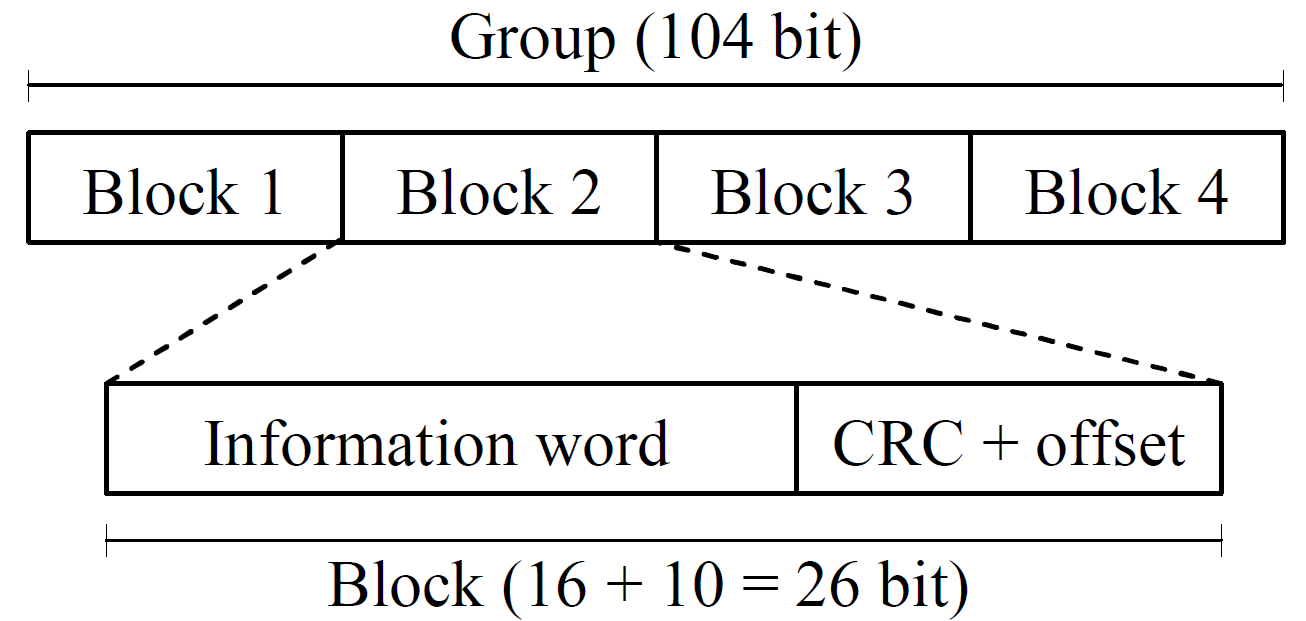
\includegraphics[width=0.4\linewidth]{RDSPack.png}
\caption{Paquetes de información RDS}
\end{figure}

\section{Resultados}
\label{S:3}
En esta sección describiré como obtuve la señal RDS usando GNURADIO, RTL2832 y Ubuntu.

\subsection{Instalación RTL}
Lo primero que se hizo es los sistemas operativos basados en debian (Ubuntu y Raspian) pudieran utilizar el RTL2832 por medio de terminal.
\begin{lstlisting}

 sudo apt-get install git cmake libusb-1.0-0-dev build-essential
 cd ~
 git clone git://git.osmocom.org/rtl-sdr.git
 cd rtl-sdr
 mkdir build
 cd build
 cmake ../ -DINSTALL_UDEV_RULES=ON -DDETACH_KERNEL_DRIVER=ON
 make
 sudo make install
 sudo ldconfig
 sudo cp ./rtl-sdr/rtl-sdr.rules /etc/udev/rules.d/ 
 cd ~
 sudo nano /etc/modprobe.d/rtl-blacklist.conf
\end{lstlisting}
Despues editar el archivon rtl-blacklist.conf
\begin{lstlisting}
blacklist dvb_usb_rtl28xxu
blacklist rtl2832

\end{lstlisting}

Para probar que se instaló correctamente escribimos ahora en terminal
\begin{lstlisting}
rtl_test -t
\end{lstlisting}
y nos debe de mostrar:

\begin{lstlisting}
 Found 1 device(s):
  0:  Generic, RTL2832U, SN: 77771111153705700

Using device 0: Generic RTL2832U
Found Rafael Micro R820T tuner
Supported gain values (29): 0.0 0.9 1.4 2.7 3.7 7.7 8.7 12.5 14.4 15.7 
16.6 19.7 20.7 22.9 25.4 28.0 29.7 32.8 33.8 36.4 37.2 38.6 40.2 42.1 
43.4 43.9 44.5 48.0 49.6
Sampling at 2048000 S/s.

Info: This tool will continuously read from the device, and report if
samples get lost. If you observe no further output, everything is fine.

Reading samples in async mode...
 \end{lstlisting}
Para sintonizar una estación de FM vía terminal:
 
 
 \begin{lstlisting}
 sudo apt-get install sox
 sudo rtl_fm -M wbfm -f 99.3M | play -r 32k -t raw -e s -b 16 
 -c 1 -V1 -
  \end{lstlisting}
  
 \begin{figure}[htbp!]
\centering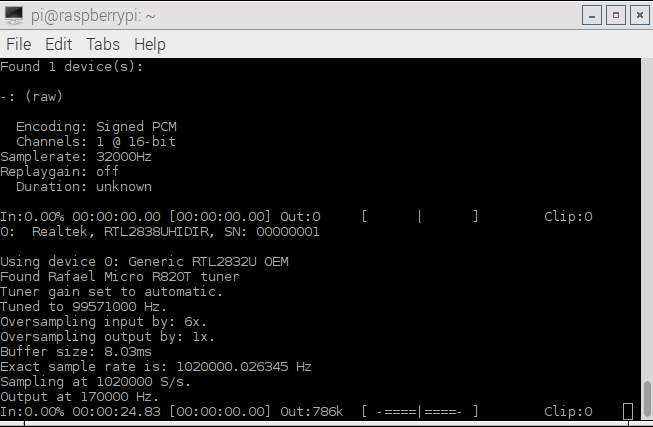
\includegraphics[width=0.7\linewidth]{terminalRadio.png}
\caption{FM en Terminal}
\label{freqRDS}
\end{figure}
  
\subsection{Instalación GNURadio en Ubuntu}
Este paso aunque a primera vista algo trivial no lo es, como es un proyecto Open Source tiene muchas formas de instalación que según se instale puede o no funcionar correctamente.
Para solo utilizar módulos básicos y proyectos menores la instalación seria


\begin{lstlisting}
sudo apt-get install gnuradio gnuradio-dev
  \end{lstlisting}
 Pero esta versión es algo inestable en especial para la generación de gráficos en WX o QT sin mencionar que utiliza una versión distinta de Volk por lo que agregar módulos tiene muchos errores.
  Después de probar otros métodos como Pybombs para la instalación decidí construir y compilar todo desde los archivos fuentes. Esto dio buenos resultados y es lo más estable para creación de módulos y manejo de hardware.

  
 
  
\subsection{RDS}
Esto es lo central del proyecto, el primer paso fue sintonizar alguna estación de FM, para esto se usa bloque RTL-SDR donde se configure la frecuencia FM, el ancho de banda de esta y la ganancia de nuestro RTL2832, para mi caso en particular dada las condiciones de ruido RF (por la cercanía a antenas celulares, redes WIFI, dispositivos Bluetooth y muros) solo dos estaciones FM eran posible sintonizar siempre que se usara una ganancia superior a 40dB. Las estaciones fueron 95.9 y 99.3.


El siguiente paso fue escuchar la estación FM, primero propuse algunos parámetros para el muestro, decimación, ancho de banda y  frecuencia de corte, como los utilizo en más de un bloque los use como variables \ref{variablesRDS} y para controlar la ganancia, volumen y estación (Frecuencia) use controles GUI \ref{controlRDS}.


 \begin{figure}[htbp!]
\centering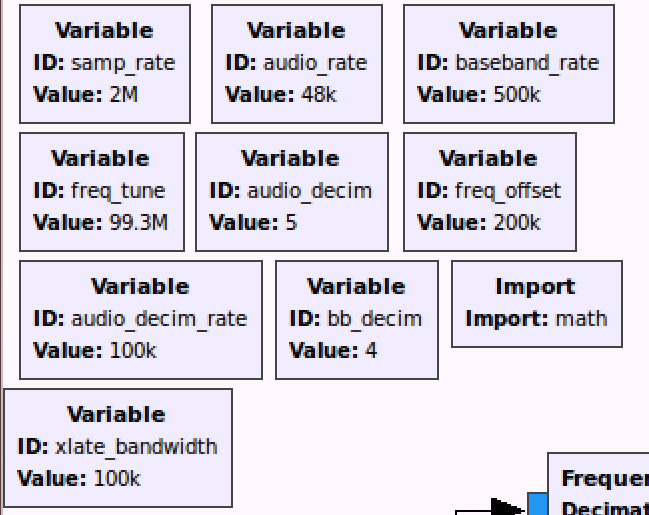
\includegraphics[width=0.35\linewidth]{variables.PNG}
\caption{Variables}
\label{variablesRDS}
\end{figure}


 \begin{figure}[htbp!]
\centering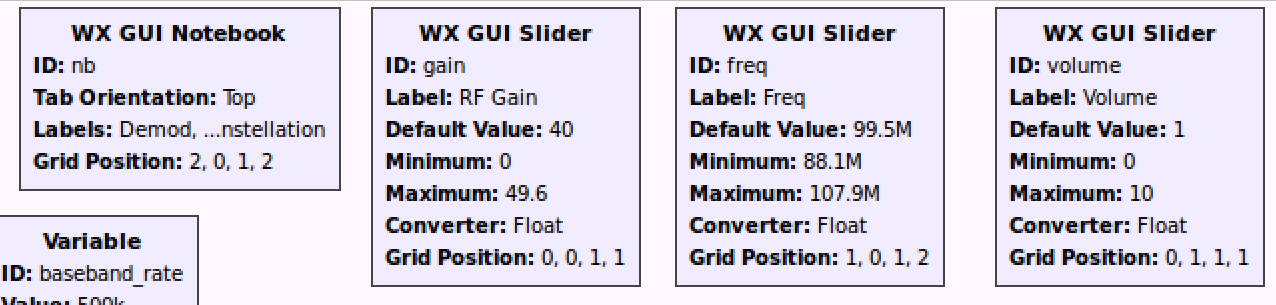
\includegraphics[width=0.5\linewidth]{GUIControls.PNG}
\caption{Controles del programa}
\label{controlRDS}
\end{figure}


  

Ahora para sintonizar la estación utilice el bloque RTL-SDR donde se configura las variables antes mencionadas, a esta señal hay que aplicarle filtro pasabajas para solo tomar el ancho de banda de la señal que necesitamos como para limpiar la señal de cualquier ruido, para esto utilice un filtro FIR pasabajas. Para la demodulación de FM utilizamos el bloque WBFM (FM de banda ancha el ideal para sistemas RDS) esto nos entrega una señal donde podemos observar, la señal FM monoaural, tono piloto, L-R,L+R (señales de estéreo) y la señal RDS centrada en los 57KHz.

 \begin{figure}[htbp!]
\centering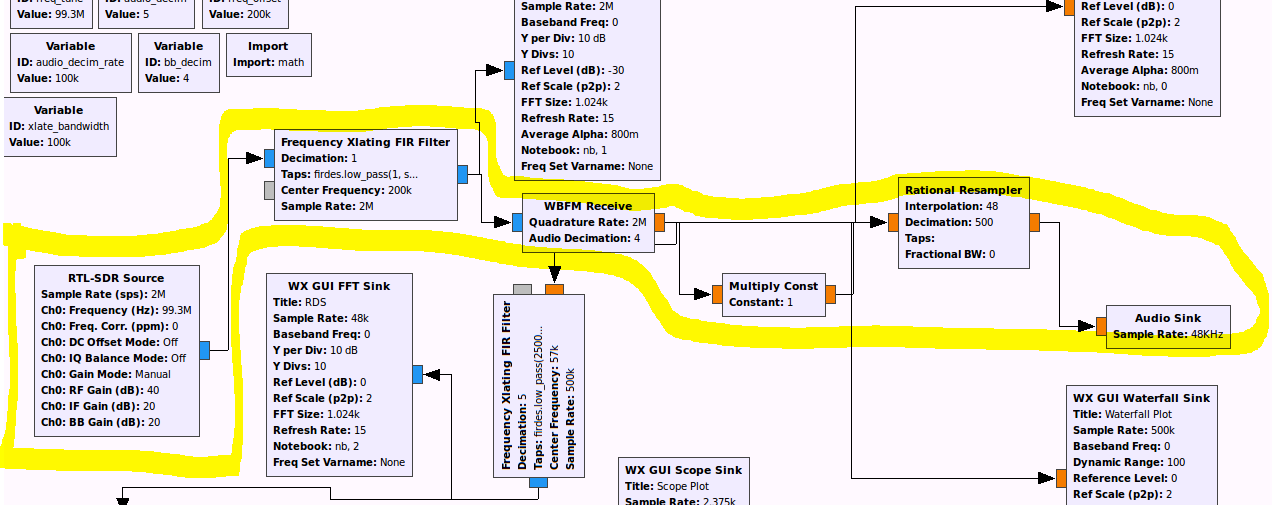
\includegraphics[width=0.7\linewidth]{FMsint.PNG}
\caption{Etapa de Radio FM}
\label{FMsint}
\end{figure}



El siguiente paso es extraer la portadora RDS de la señal FM demodulada, por lo que se aplica otro filtro FIR pasabajas centrado en 57 KHz, para demodularla a una señal digital. Para esto se usa una técnica llamada "Matched Filter".

 \begin{figure}[htbp!]
\centering\includegraphics[width=0.7\linewidth]{RDSMark.PNG}
\caption{Etapa de procesamiento RDS}
\label{RDSMark}
\end{figure}


El Matched filter es necesario para obtener una señal cuadrada, primero usamos el metodo "root-raised-cosine filter" para sincronizar estos pulsos hay varias técnicas para hacer algo llamado "Costas loop" para esta aplicación se usó un demodulador MPSK, ya en este punto podemos observar la constelación de la modulación. Posteriormente procedemos a hacer un threshold para crear una señal binaria, que se va acumulando en paquetes de bits. Estos son decodificados con dos bloques el primero utiliza código Manchester y va tomando los 16 bits de información de cada bloque del protocolo RDS. A continuación toma las palabras decodificadas y hace una búsqueda en LUTs de su significado estos dos bloques están C++ creados para otra plataforma de SDR, pero utilizables en GNURADIO y por ultimo van a un bloque de exhibición creado en Python y WX,en las siguientes figuras muestro capturas de pantalla del GUI, las estaciones locales solo transmiten el nombre de estas, pero la plantilla del programa permite extraer y desplegar más información.
  \begin{figure}[htbp!]
\centering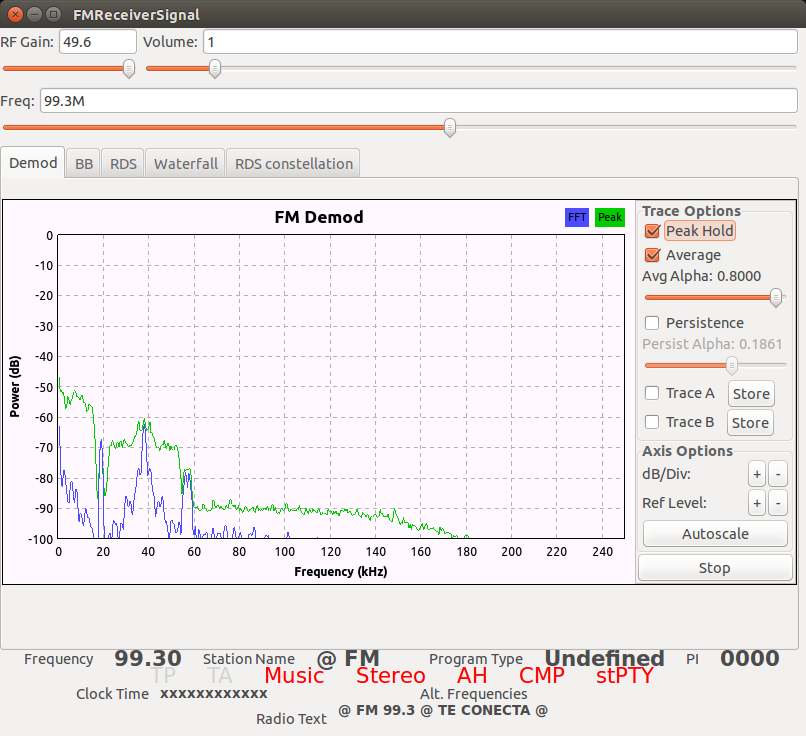
\includegraphics[width=0.7\linewidth]{ffdemod.png}
\caption{demodulación FM}
\label{demodFM}
\end{figure}

  \begin{figure}[htbp!]
\centering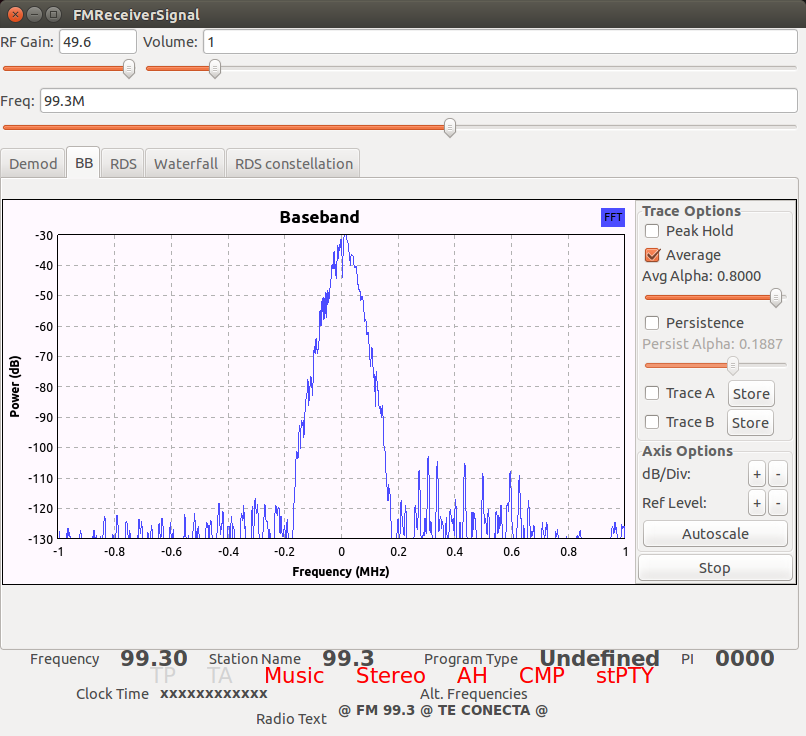
\includegraphics[width=0.6\linewidth]{bbfm.png}
\caption{Banda Base FM}
\label{bbFM}
\end{figure}

  \begin{figure}[htbp!]
\centering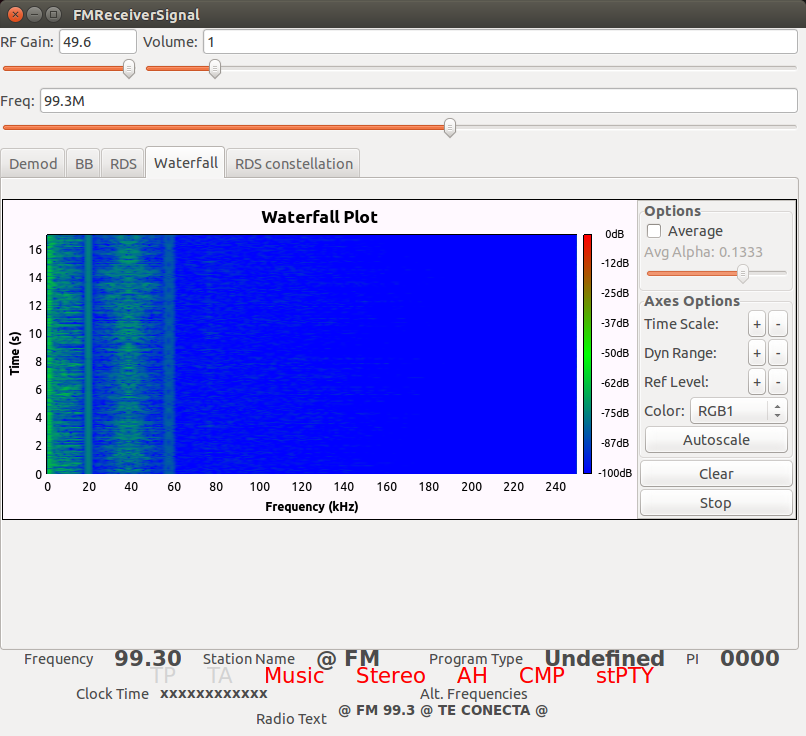
\includegraphics[width=0.6\linewidth]{waterfallfm.png}
\caption{Grafico de Cascada FM}
\label{waterfallFM}
\end{figure}

  \begin{figure}[htbp!]
\centering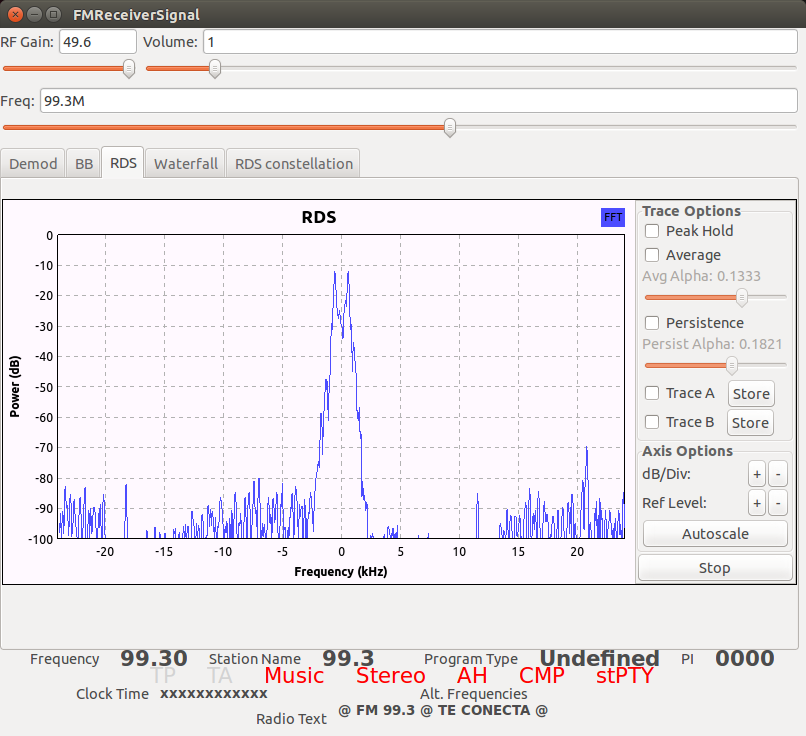
\includegraphics[width=0.6\linewidth]{rdsfm.png}
\caption{RDS FM}
\label{rdsFM}
\end{figure}


  \begin{figure}[htbp!]
\centering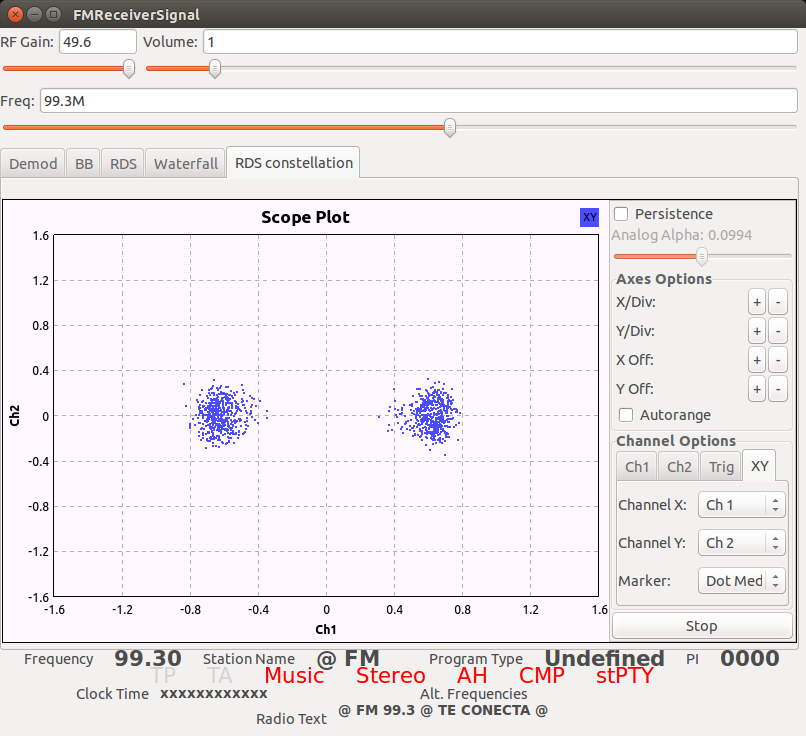
\includegraphics[width=0.6\linewidth]{constelacion.png}
\caption{Constelación RDS}
\label{constell}
\end{figure}



\subsection{GNURADIO en Raspberry PI}
Se intentó ejecutar estos códigos en una computadora Raspberry PI, utilice el OS Raspbian, pero es aqui donde me topé con varias dificultades que me mostraron las debilidades del proyecto GNURADIO, que van desde la instalación. Via apt-get las versión de GNURADIO es una muy anterior a la actual (3.7.5 actual 3.7.9), así que opte por construir y compilar GNURADIO en Raspberry Pi, esto toma alrededor de 48 horas de procesamiento, si aumenta la memoria SWAP al máximo (2GB) se reduce a 24 horas. También intente la instalación via Pybombs que toma otras 24 horas.
Una vez instalado hice pruebas de sintonización FM si funcionaron, pero por capacidad de procesamiento solo era viable observar un GUI, así como no reproduce audio ya que hay errores con la librería gqrx, módulos como "root-raised-cosine filter" no están disponibles y tiene errores con la creación de módulos. Revisando de manera más detallada la documentación de GNURADIO Raspberry PI no es la plataforma para aplicaciones de SDR, se recomiendan plataformas como blade de HackRF pero estas plataformas tienen un costo de más de \$ 400.00 dólares. Por lo que a manera personal recomiendo plataformas basadas en PC que pueda ejecutar cualquier versión de Ubuntu superior a la 10.4.


%\section{Observaciones}
%\label{S:4}



%% The Appendices part is started with the command \appendix;
%% appendix sections are then done as normal sections
%% \appendix

%% \section{}
%% \label{}

%% References
%%
%% Following citation commands can be used in the body text:
%% Usage of \cite is as follows:
%%   \cite{key}          ==>>  [#]
%%   \cite[chap. 2]{key} ==>>  [#, chap. 2]
%%   \citet{key}         ==>>  Author [#]

%% References with bibTeX database:


\bibliographystyle{model1-num-names}
\bibliography{sample.bib}

%% Authors are advised to submit their bibtex database files. They are
%% requested to list a bibtex style file in the manuscript if they do
%% not want to use model1-num-names.bst.

%% References without bibTeX database:

% \begin{thebibliography}{00}

%% \bibitem must have the following form:
%%   \bibitem{key}...
%%

% \bibitem{}

% \end{thebibliography}


\end{document}

%%
%% End of file `elsarticle-template-1-num.tex'.